
\chapter{CTMQC}
\label{chap:CTMQC}


\section{Exact Factorisation}
CTMQC comes from taking the semi-classical limit of an exact factorisation of the molecular wavefunction into its constituent electronic and nuclear components \cite{abedi_exact_2010}. Where the electronic component is parametrically dependent on the nuclear coordinates, $\textbf{R}$. This is shown below in eq \eqref{eq:exact_fact} where $\chi$ is the nuclear wavefunction and $\Phi$ is the electronic one.
\begin{equation}
 \Psi(\textbf{R}, \textbf{r}, t) = \Phi_{\textbf{R}}(\textbf{r}, t) \chi(\textbf{R}, t)
 \label{eq:exact_fact}
 \end{equation}
In the above equation (and throughout this report) I will denote nuclear coordinates and electronic coordinates $R$ and $r$ respectively. The nuclear and electronic wavefunctions then obey separate, but coupled, time-dependent schr\"odinger equations for spatial and temporal evolution. This representation has proven to be useful in furthering understanding through exact solutions of small toy-model systems \cite{agostini_quantum-classical_2016, gossel_coupled-trajectory_2018}. However, in this report I will be focussing on the semi-classical limit of these equations (CTMQC) and give some early results of a combination of this and the AOM method explained previously in section \ref{chap:FOB}.
The equations for the evolution of the electronic and nuclear wavefunctions in the exact factorisation \cite{abedi_exact_2010} are given below:
\begin{align}
  i\hbar \frac{\delta}{\delta t} \Phi_{\textbf{R}}(\textbf{r}, t) &= \left( \hat{H}_{BO} + \hat{U}_{en}\left[ \Phi_{\textbf{R}}, \chi\right] - \epsilon(\textbf{R}, t) \right) \Phi_{\textbf{R}} (\textbf{r}, t)
  \label{eq:electronic_exact}
\\
i\hbar \frac{\delta}{\delta t} \chi (\textbf{R}, t) &= \left( \sum_{\nu = 1}^{N_{n}} \frac{[-i\hbar\nabla_{\nu} + \textbf{A}_{\nu}(\textbf{R}, t)]^2}{2 M_{\nu}} + \epsilon(\textbf{R}, t)\right) \chi (\textbf{R}, t)
  \label{eq:nuclear_exact}
\end{align}
Where $\hat{H}_{BO}$ is the Born-Oppenheimer Hamiltonian, that is $\hat{T}_{e} + \hat{W}_{ee} + \hat{W}_{nn} + \hat{V}_{en}$. Where $\hat{T}_{e}$ is the electronic kinetic energy operator, $\hat{W}_{ee/nn}$ is the electron-electron/nuclei-nuclei interation and $V_{en}$ is the electronic-nuclear potential.
\\\\
The $\hat{U}_{en}$ is an electronic-nuclear coupling operator (ENCO). This is defined as \begin{equation}
  \hat{U}_{en}[\Phi_{\textbf{R}}, \chi] = \sum_{\nu=1}^{N_{nuc}} \frac{1}{M_{\nu}} \left[ \frac{\left[-i \hbar \nabla_{\nu} - \textbf{A}_{\nu}(\textbf{R}, t) \right]^2}{2} + \left( \left. \left. \frac{-i\hbar \nabla_{\nu} \chi}{\chi} + \textbf{A}_{\nu}(\textbf{R, t})\right)\right( -i\hbar\nabla_{\nu} - \textbf{A}_{\nu}(\textbf{R}, t)\right) \right]
  \label{eq:ENCO}
\end{equation}
\\
Where the $\textbf{A}_{\nu}$ is a time-dependent vector potential (TDVP), given by $\left\langle \Phi_{\textbf{R}}(t) \right\vert \left. - i \hbar \nabla_{\nu} \Phi_{\textbf{R}} \right\rangle_{\textbf{r}}$ and $M_{\nu}$ is the mass of nuclei $\nu$.
Finally $\epsilon(\textbf{R}, t)$ is a time-dependent scalar potential energy surface (TDPES), given by $\langle \Phi_{\textbf{R}}(t) \vert \hat{H}_{BO} + \hat{U}_{en}^{coup} - i\hbar \frac{\delta}{\delta t} \vert \Phi_{\textbf{R}}(t) \rangle_{\textbf{r}}$.
\\
\begin{wrapfigure}{r}{0.5 \textwidth}
  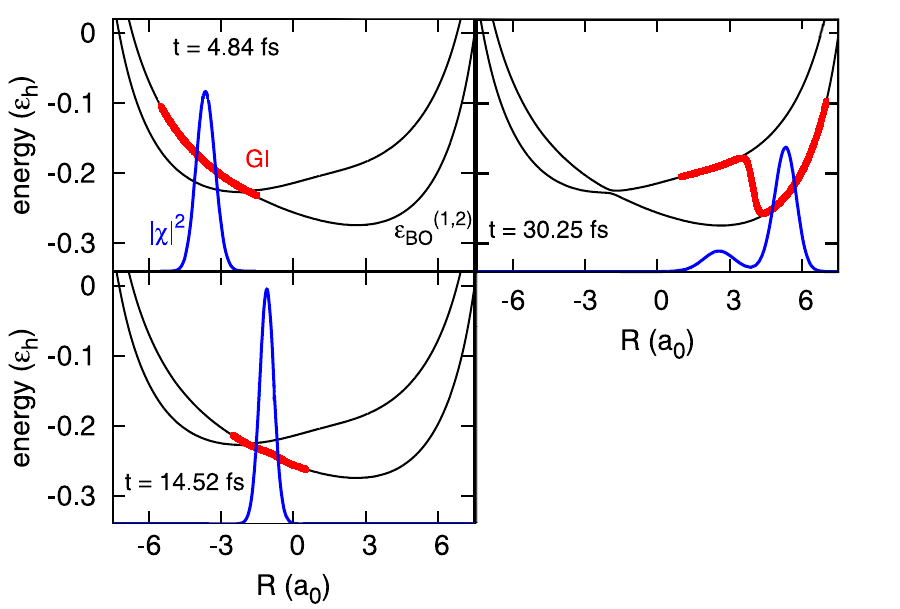
\includegraphics[width=0.5\textwidth]{./img/nuclear_splitting_TDPES.png}
  \caption{A demonstration of how the TDPES can cause the splitting of the nuclear wavepacket in non-adiabatic regions. The red line represents the TDPES and the blue is the nuclear density. Adapted from \cite{agostini_exact_2015} \label{fig:step_TDPES}}
\end{wrapfigure}
\\
The effects of the TDPES, TDVP and the ENCO have been investigated in multiple works \cite{agostini_semiclassical_2015, agostini_exact_2015, agostini_mixed_2013, abedi_dynamical_2013, Min2014Dec}. The TDPES and TDVP are both responsible for the evolution of the system
\cite{agostini_semiclassical_2015}.  The TDPES provides exact classical forces on the nuclei. In fact, an alternative independent-trajectory semi-classical scheme has been investigated using these exact forces \cite{agostini_exact_2015}. This found the TDPES is responsible for the splitting of the nuclear wavepacket in regions of high non-adiabaticity by taking the shape of a step function between the 2 adiabatic potentials. This is demonstrated in figure \ref{fig:step_TDPES}. Finally the electronic-nuclear coupling operator (ENCO) is responsible for other non-adiabatic effects in the system such as electronic nonadiabtic transitions and decoherence \cite{agostini_semiclassical_2015}.
\section{Approximations in CTMQC}
Six approximations have been made in the derivation of CTMQC, these are discussed in detail in Ref. \cite{agostini_quantum-classical_2016}. In the interest of completeness I have summarised them below.
\subsection{Classical Nuclei}
Techniques that include nuclear quantum effects (NQEs); such as multiple spawning \cite{Martnnez*2005Oct}, ring-polymer surface hopping \cite{Shakib2017Jul} and nonadiabatic Bohmian dynamics \cite{Curchod2011Feb, Tavernelli2013Apr} although extremely accurate, cannot be applied to hundreds or thousands of molecules. This is due to their high computational cost. Further, in many systems of interest NQEs are negigible, especially at room temperature. For this reason the classical limit of the nuclear Schr\"odinger equation \eqref{eq:nuclear_exact} is taken when deriving the CTMQC equations.
\subsection{Neglect the ENCO in the TDPES}
The electron-nuclei coupling operator is omitted in the expression for the time-dependent potential energy surface. This is justified as the first term ($\left[-i \hbar \nabla_{\nu} - \textbf{A}_{\nu}(\textbf{R}, t) \right]^2$) contains a second order derivative which is expensive to calculate and has a neglible effect compared to the second term in the ENCO \cite{Scherrer2015Aug}. However, the rest of the ENCO is equal to zero when averaged over $\Phi_{\textbf{R}}(\textbf{r},t)$ so it does not contribute to the TDPES.
\subsection{Derivative of the Adiabatic Coefficients}
The derivative of the adiabatic coefficients appears in the electronic evolution equations. However, we can re-write the derivative of the adiabatic coefficients in terms of their modulus and phase:
\begin{equation}
  \nabla_{\nu} C_{l}^{(I)}(t) = \left[ \underbrace{\frac{\nabla_{\nu} |C_{l}^{(I)}(t)|}{|C_{l}^{(I)}(t)|}}_{(\text{Term 1})} + \underbrace{\frac{i}{\hbar} \nabla_{\nu} \gamma_{l}^{(I)}(t)}_{(\text{Term 2})}\right] C_{l}^{(I)}(t)
\end{equation}
It has been found that the first term is negligible compared to the second \cite{abedi_dynamical_2013, agostini_mixed_2013, agostini_exact_2015} so it doesn't need to be calculated and we can remove it. It was also assumed that the NACVs are localised in space meaning that, after some algebra, the spatial derivative of the adiabatic coefficient can be written as:
\begin{equation}
  \nabla_{\nu} C_{l}^{(I)}(t) = \frac{i}{\hbar} \nabla_{\nu} \gamma_{l}^{(I)}(t) C_{l}^{(I)}(t) = -\frac{i}{\hbar} \int^{t} dt' \nabla_{\nu} \epsilon_{l}^{(I)} C_{l}^{(I)}(t) = -\frac{i}{\hbar} \textbf{f}_{l}^{(I)} C_{l}^{(I)}(t)
  \label{eq:hist_force}
\end{equation}
Where $\epsilon_{l}^{(I)}$ is the energy of the l$^{th}$ adiabatic potential energy surface for trajectory I, $C_{l}^{(I)}$ is the adiabatic expansion coefficient for state l and trajectory I. The $\textbf{f}_{l}^{(I)}$ is the time-integrated adiabatic force.
\subsection{Gaussian Nuclear Wavepackets}
In order to calculate the quantum momentum -the new term in CTMQC. Knowledge of the nuclear distribution is needed. To this end the nuclear wavepacket is assumed to take the shape of a Gaussian. This is centred on the atomic coordinate with a width $\sigma$. In this work I have used a constant width throughout, with plans to implement dynamic Gaussian width calculations later. However, the nuclei are still propagated classically, the width parameter is only used in the calculation of the quantum momentum.
\subsection{Seperating the Effects of Decoherence and NACVs}
So as to not introduce any population transfer (due to the quantum momentum) when the NACV is zero a fifth approximation has been introduced. Namely the quantum momentum depends on pairs of states -l,k. This enables the seperation of the `competing' effects of the NACV and the Quantum Momentum.
\section{The CTMQC equations}
\subsection{Adiabatic Basis \label{sec:ad_eqns}}
The equations for the propagation of the classical nuclei and the expansion coefficients in the CTMQC framework in the adiabatic basis are given below:
\begin{dmath}
  \dot{\textbf{P}}_{\nu}^{(I)} =
  -\overbrace{
     \sum_{k} |C_{k}^{(I)}|^2 \nabla_{\nu}\epsilon_{k}^{(I)}
     - \sum_{k,l} C_{l}^{(I)} C_{k}^{* (I)} \left(\epsilon_{k}^{(I)}  - \epsilon_{l}^{(I)}   \right)
  }^{\text{Ehrenfest}}
  \\
  \underbrace{
    - \sum_{l,k} |C_{l}^{(I)}|^2 \left( \sum_{\nu'=1}^{N_n}    \frac{2}{\hbar M_{\nu'}} \mathcal{Q}_{lk, \nu}^{(I)} \cdot    \textbf{f}_{l, \nu}^{(I)} \right)\left[ |C_{k}^{(I)}|^2    \textbf{f}_{k,\nu}^{(I)} - \textbf{f}_{l,\nu}^{(I)} \right]
  }_{\text{Quantum Momentum}}
    \label{eq:nuc_adiab}
\end{dmath}

\begin{dmath}
  \dot{C}_{l}^{(I)} =
  \overbrace{
    -\frac{i}{\hbar} \epsilon_l^{(I)} C_{l}
    - \sum_k C_k^{(I)} d_{lk}^{ad \ (I)}
  }^{\text{Ehrenfest}}
  \\
  \underbrace{
    - \sum_{\nu=1}^{N_n}\sum_{k} \frac{\mathcal{Q}_{lk, \nu}^{(I)}}{\hbar M_\nu} \cdot \left[ \textbf{f}_{k,\nu}^{(I)} - \textbf{f}_{l,\nu}^{(I)} \right] |C_{k}^{(I)}|^2 C_{l}^{(I)}
  }_{\text{Quantum Momentum}}
  \label{eq:elec_adiab}
\end{dmath}
Where the $\epsilon_k$ term is the potential energy on the k$^{th}$ potential energy surface. $C_l$ is the adiabatic expansion coefficient corresponding to the l$^{th}$ state. The sum over k and l indicates a sum over all states, the (I) superscript is a replica index and the $\nu$ is an atom index. $M_{\nu}$ is the nuclear mass and $d_{lk}{^(I)}$ represents the non-adiabatic coupling element (in the adiabtic basis) between adiabatic states l and k, $\langle \psi_{l} \vert \frac{d}{dt}\psi_{k} \rangle$.
The 2 new terms in this scheme not seen in other one are the $\mathcal{Q}_{lk, \nu}^{(I)}$ and the $\textbf{f}_{k, \nu}^{(I)}$. These are the quantum momentum and the history dependent adiabatic force. The history dependent force in defined in equation \eqref{eq:hist_force} this keeps a record of the previous forces in the system. The quantum momentum term couples the trajectories together (making this a coupled-trajectory scheme). Together the history dependent force and quantum momentum are responsible for the decoherence in the `Quantum Momentum' parts of the
above equations \cite{gossel_coupled-trajectory_2018}. Notably, although these equations have been derived from the exact factorisation equations separately from Ehrenfest they do contain exactly the Ehrenfest equations within them (marked `Ehrenfest'). This scheme can therefore be seen as an Ehrenfest scheme with a correction that captures branching of the nuclear wavefunction and decoherence within it.
\\\\
We can also see in equation \eqref{eq:elec_adiab} if we are in a pure adiabatic state i.e. all population on a single adiabatic state, there is no contribution from the quantum momentum part of the equations. In this scenario the evolution equations become simply Ehrenfest equations. For example, if we only have 1 state in the system with non-zero adiabatic population then the term $|C_{k}^{(I)}|^2 C_{l}$ is only non-zero when $l = k$. However, when $l = k$, the term $\left[ \textbf{f}_{k,\nu}^{(I)} - \textbf{f}_{l,\nu}^{(I)} \right]$ is zero as $\textbf{f}_{k,\nu}^{(I)} = \textbf{f}_{l,\nu}^{(I)}$.
Therefore, the quantum momentum term can be seen to only kick in when there is a mixing of adiabatic states. In the adiabatic formulation of these equations it is the adiabatic NACV $\textbf{d}_{lk, \nu}^{ad, (I)}$ that is responsible for the initial mixing of the populations from pure adiabatic states.

\subsection{Diabatic Basis}
The equations above \eqref{eq:nuc_adiab} \& \eqref{eq:elec_adiab} are both in the adiabatic basis. However, to make use of the FOB-formalism detailed in section \ref{chap:FOB} already implemented in the CP2K software package \cite{CP2K} these need to be transformed to the orthogonal diabatic basis, $\phi$. After applying the transformation matrix $\mathbb{U}$ and some algebra the equations in the diabatic basis can be written as:
\begin{dmath}
{ F_{v}^{(I)}(t)} =
\overbrace{ -\sum_{l,k} u_{l}^{(I) *} u_{k}^{(I)} \nabla_{v} H_{lk}^{(I)} - \sum_{l,k,a} d_{la}^{(I)}H_{ak}^{(I)} - d_{ak}^{(I)}H_{la}^{(I)}}^{\text{Ehrenfest}}
\\
 - \underbrace{2 \sum_{l} |C_{l}^{(I)}|^2 \sum_{n} \left( \sum^{N}_{\nu'} \frac{\mathcal{Q}^{(I)}_{ln,v'}(t)}{\hbar M_{v'}} \cdot \textbf{f}^{(I)}_{l,v'}\right)\left[  |C_{n}^{(I)}|^{2} \textbf{f}^{(I)}_{n,v} - \textbf{f}^{(I)}_{l,v} \right]}_{\text{Quantum Momentum}}
 \label{eq:diab_force}
\end{dmath}

\begin{align}
\dot{u}_k^{(I)} =
&\overbrace{ - \frac{i}{\hbar}\sum\limits_{l} u_l^{(I)} \left(H_{kl}^{(I)} + i \hbar d_{kl}^{(I)} \right) }^{\text{Ehrenfest}} \\
& + \underbrace{\sum_{s} U_{ks} \sum_{\nu = 1}^{N_n} \sum_n   \frac{\mathcal{Q}_{sn,\nu}^{(I)}}{\hbar M_\nu}\cdot \left[ \mathbf{f}_{n, \nu}^{(I)}- \mathbf{f}^{(I)}_{s, \nu}\right]\vert C_n^{(I)} \vert^2 \sum_{l} U^{*}_{sl} u^{(I)}_{l}}_{\text{Quantum Momentum}}
\label{eq:diab_elec}
\end{align}
Where $u_l^{(I)}$ represents the diabatic expansion coefficient for (orthogonal) diabatic state l on trajectory I. $H_{kl}^{(I)} = \langle \phi_{k}^{(I)} | H^{(I)} | \phi_{l}^{(I)} \rangle$ is the diabatic Hamiltonian. $d_{kl} = \langle \phi_{k}^{(I)} | \dot{\phi_{l}^{(I)}} \rangle$ is the diabatic non-adiabatic coupling element (NACE). $U_{ks} = \langle \phi_{k} | \psi_{s} \rangle $
is the adiabatic-diabatic transformation matrix. The other terms have been previously defined (see section
 \label{sec:ad_eqns}).
 \\\\
 The 2 expressions can again be decomposed into a quantum momentum part and an Ehrenfest part. In the force expression \eqref{eq:diab_force} the Ehrenfest part comprises 2 terms. In tests I have found the first term  contributes significantly more to the overall force than the second `commutator' term. This means that the second term, can be neglected in most situations. The quantum momentum term in the force expression is expressed in the adiabatic basis. This is because it is basis independent and numerically transforming it with transformation matrices would result in unnecessary computation. The quantum momentum part of the electronic equation \eqref{eq:diab_elec} is largely unchanged compared to the adiabatic one \eqref{eq:elec_adiab} and an on-the-fly transformation from adiabatic to diabatic representations is required during propagation.
 \\\\
 The diabatic hamiltonian, as opposed to the adiabatic one, now contains non-zero off-diagonal elements. This is the primary term responsible for population transfer when in pure adiabatic states. The diabatic NACE has a much smaller effect.
 \section{Calculating the Quantum Momentum \label{sec:calc_QM}}
 The technique for calculating the quantum momentum term is outlined in detail in the SI of \cite{min_ab_2017}. The original equations given in \cite{agostini_quantum-classical_2016} present a quantum momentum term without state indices (l,k). This, due to approximations made in the derivation of CTMQC, results in population transfer even when the non-adiabatic couplings between states are zero. Therefore Agostini et al has enforced this with the pair-wise state dependence of the quantum momentum.
 \\\\
The quantum momentum is defined as:
\begin{equation}
  \mathcal{Q}_{\nu}{(I)} = \frac{-\hbar \nabla_{\nu} |\chi^{(I)}|}{|\chi^{(I)}|} \frac{-\hbar \nabla_{\nu} |\chi^{(I)}|^2}{2|\chi^{(I)}|^2}
  \label{eq:QM_def}
\end{equation}
In order to reconstruct the nuclear density Gaussian distributions can be used. This results in a linear expression for the quantum momentum.
The full details of the derivation are given in the supplementary information of \cite{min_ab_2017}. The resulting linear expression for the quantum momentum is given below:
\begin{equation}
  \mathcal{Q}_{lk, \nu}^{(I)} = \alpha_{\nu}^{(I)} \textbf{R}_{\nu}^{(I)} - \textbf{R}_{lk, \nu}
  \label{eq:QM_lin}
\end{equation}
Where $\textbf{R}_{\nu}^{(I)}$ are the nuclear coordinates on trajectory I on atom $\nu$. The $\alpha_{\nu}{^(I)}$ term is a weighted average over trajectories of the product of the gaussian's assigned to each atomic coordinate, i.e:
\begin{equation}
  \alpha_{\nu}^{(I)} = \sum_{J}^{N_{tr}} \frac{\hbar \prod_{\nu'} g_{\sigma_{\nu'}^{(J)}(t)}\left(\textbf{R}_{\nu'}^{(I)}(t) - \textbf{R}_{\nu'}^{(J)}(t)\right)}   {2 \sigma_{\nu}^{(J)}(t)^2\sum_{K}^{N_{tr}}\prod_{\nu'} g_{\sigma_{\nu'}^{(K)}(t)}\left(\textbf{R}_{\nu'}^{(I)}(t) - \textbf{R}_{\nu'}^{K)}(t)\right)}
  \label{eq:alpha}
\end{equation}
Where $\sigma_{\nu'}^{(J)}(t)$ is a width parameter for the width of the gaussian centered at atomic coordinates. Along with the $\textbf{R}_{lk, \nu}$ term the $\alpha_{\nu}^{(I)}$ performs the job of coupling the trajectories together. The $\textbf{R}_{lk, \nu}$ term also given in the SI of \cite{min_ab_2017} is defined for each cartesian dimension as:
\begin{equation}
  R_{lk, \nu} = \sum_{I}^{N_{tr}} R_{\nu}^{(I)}(t) \alpha_{\nu}^{(I)}(t) \frac{|C_{k}^{(I)}(t)|^2 |C_{l}^{(I)}(t)|^2 \left( f_{k, \nu}^{(I)}(t) - f_{l, \nu}^{(I)}(t) \right)}{\sum_{J} |C_{k}^{(J)}(t)|^2 |C_{l}^{(J)}(t)|^2 \left( f_{k, \nu}^{(J)}(t) - f_{l, \nu}^{(J)}(t) \right)}
  \label{eq:Rlk}
\end{equation}
Where the bold notation for vectors has been replaced by normal font indicating that this applies to each cartesian dimension independently. Further, in this expression $R_{lk, \nu}$ is anti-symmetric, $R_{lk} = R_{kl}$ meaning that $Q_{lk} = Q_{kl}$. At first sight the $R_{lk}$ term seems to be another weighted average. However, this isn't quite the case as the denominator can have negative terms. This causes equation \eqref{eq:Rlk} to be very sensitive to errors in the calculation of the denominator of this fraction. Any inaccuracies can lead to the denominator approaching zero faster than the numerator causing large spikes in the quantum momentum term.

\section{Testing my Implementation}
I have implemented a serial version of this algorithm in the CP2K software package \cite{CP2K}. As well as many numerical tests on individual terms in the equations, I have implemented some physical tests too. In this section I will outline some of the key tests I have performed on both the Ehrenfest part of the equations and the full CTMQC equations.
\subsection{Rabi Oscillation}
Rabi Oscillation can be shown to occur in systems that have fixed nuclear geometries (see section \ref{ap:Rabi}). During Rabi oscillation the electronic dynamics are given by an analytic formula. This can be solved in Python and used to test the implementation of the electonic propagation, decoupled from nuclear dynamics. In this test Ehrenfest was used to propagate the system, which consisted of a trimer of an Ethylene-like molecule with 10 replicas. Each of the replicas were initialised with different positions. The electronic propagation of Ehrenfest is the same as that of trajectory surface hopping so I have adapted a previously implemented subroutine from the FOB-SH method \cite{spencer_fob-sh:_2016} to work for many replicas. The results are shown in figure \ref{fig:Rabi}.
\begin{figure}[H]
  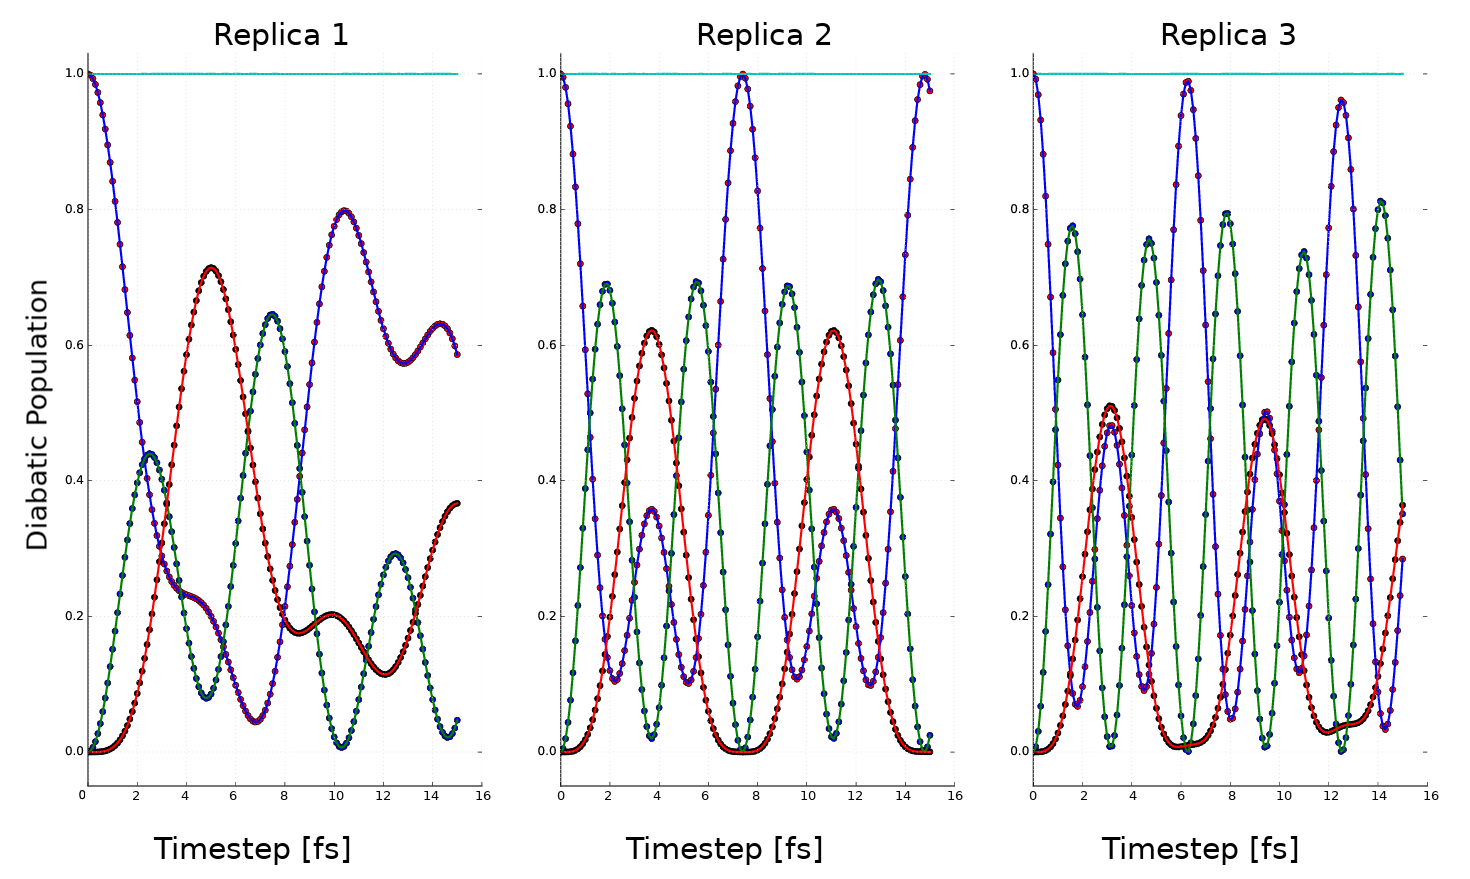
\includegraphics[width=\textwidth]{./img/3_reps_RABI.png}
  \caption{\label{fig:Rabi}Rabi oscillation for a trimer of Ethylene, results shown for 3 replicas. Solid lines indicate the output of the CP2K propagation and dots indicate the result of the analytic Rabi formula. Different colors indicate different states. The cyan line shows the sum of the diabatic populations i.e. the norm.}
\end{figure}
\noindent We can see in figure \ref{fig:Rabi} CP2K gives the same output as the analytic result. This means for Ehrenfest the electronic propagation is working as expected. Molecules in replica 1 were initialised further apart than those of replica 2 and replica 3, with replica 3 having the closest molecules. We can see that the frequency of oscillation of charge between molecules that are further apart is slower. Something we would expect to see in a realistic system. Further the new implementation of multiple replicas can be seen to work with all replicas give correct results.
\\
\subsection{Energy Conservation}
The Ehrenfest equations can be shown to conserve the potential energy + total kinetic energy \cite{john_c._tully_nonadiabatic_1998}. The potential energy is given by the effective potential (i.e. $\sum_{l} \vert C_{l}^{(I)} \vert^2 \epsilon_{l}$) and the total kinetic energy is given as a sum of the kinetic energy over all atoms. In this test the commutator term was neglected from equation \eqref{eq:diab_force}. 8 simulations were performed. These used the same initial conditions but varied a random number generator seed, which is used in the calculation of the NACVs. In each simulation 100 replicas were used over various couplings and averaged to get the average energy drift per replica. The error bar was obtained from the average energy drifts of the 8 simulations.
\begin{figure}[H]
  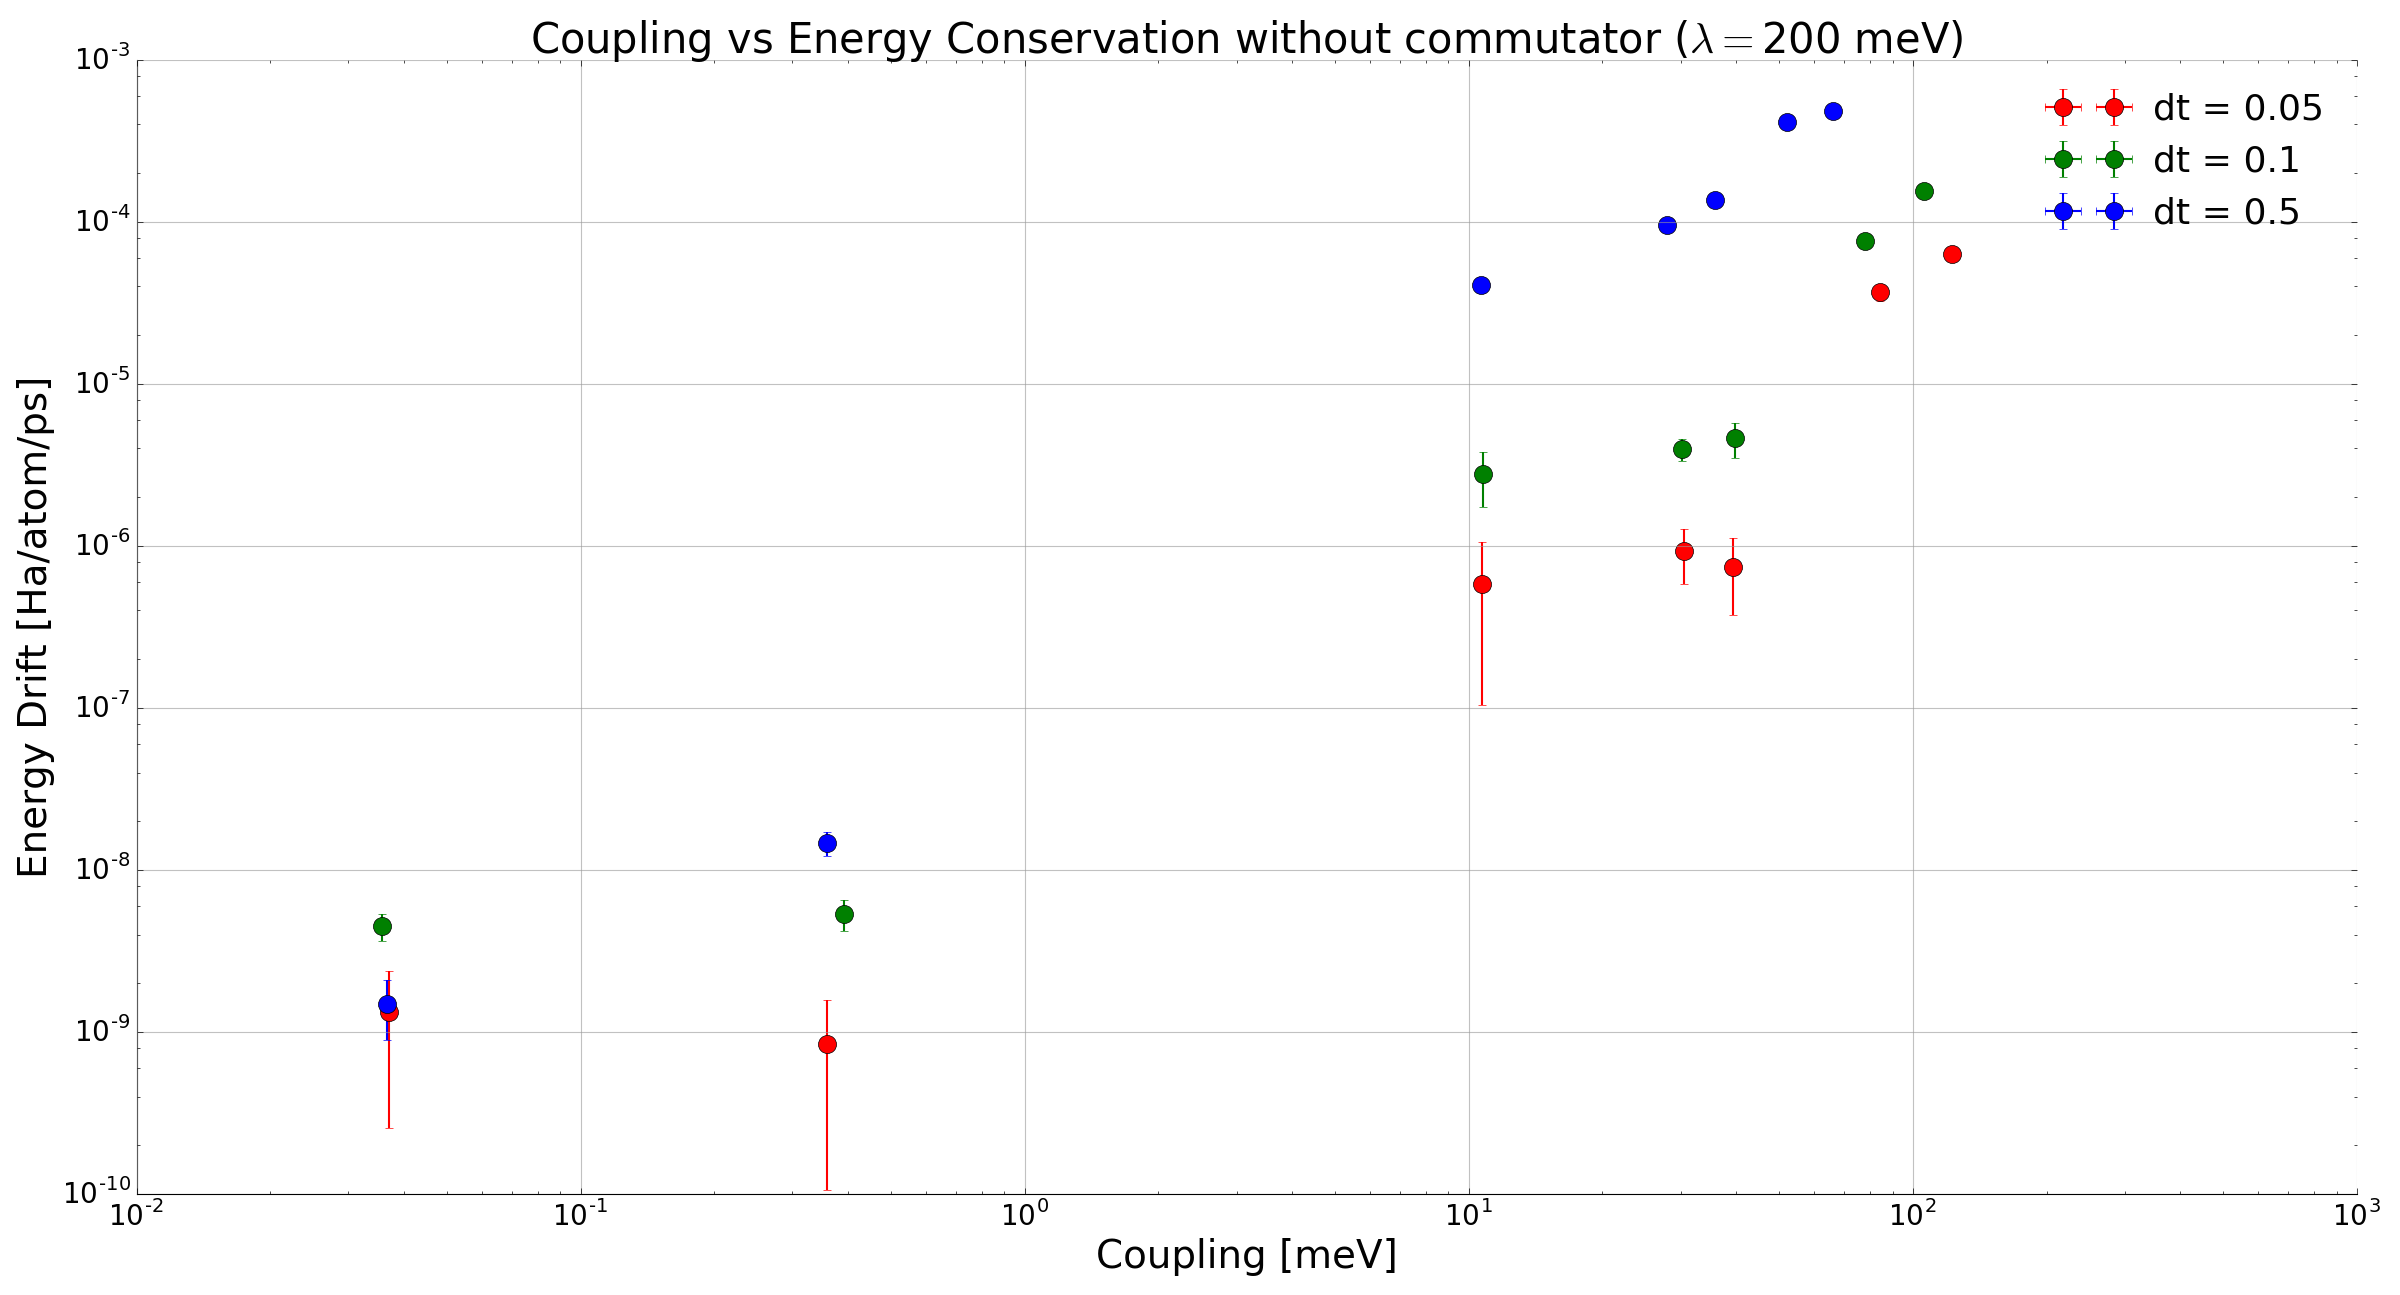
\includegraphics[width=\textwidth]{./img/energy_conservation.png}
  \caption{\label{fig:Ehren_Ener_Cons}Energy drift in Ehrenfest for various couplings. Each color represents a different nuclear time-step used in fs.}
\end{figure}
We can see that the energy is conserved very well for low couplings and starts to increase for higher ones. The exact reason for this is not known. It may be due to the fact the the effective potential energy surface is a population weighted average. If the energies are closer together around the crossing region (as in lower coupling systems) then this average becomes a better representation of the true potential. When the states are further apart the average becomes more of an approximation. From this graph a time-step of 0.1fs was chosen as a compromise between accuracy and computational cost.
\\
\subsection{Norm Conservation}
The norm of the coefficients should be conserved when propagating the equations. To not do so would mean that the total number of charge carriers is changing, i.e. electrons/holes being destroyed or created. Both the CTMQC and Ehrenfest electronic equations can be shown to conserve the norm (see appendix \ref{ap:Norm_Pres}). When propagating Ehrenfest dynamics this is very well conserved, with norm drifts (using a nuclear time-step of 0.1fs) on the order $10^{-10}$ ps$^{-1}$. However, in CTMQC the story is slightly different.
\\\\
The quantum momentum appears in both the nuclear force equation and the electronic equation. However, its current formulation using Gaussian distributions to model the nuclear density results in equation \eqref{eq:QM_lin}. That is $\mathcal{Q}_{lk,\nu}^{(I)} = \alpha_{\nu}^{(I)}\textbf{R}^{(I)}_\nu - \textbf{R}^{(I)}_{lk, \nu}$. Where the $\textbf{R}^{(I)}_{lk, \nu}$ term is calculated via equation \eqref{eq:Rlk}. This is given again below in a condensed form:
\[\textbf{R}_{lk, \nu} = \sum_{I}^{N_{tr}} R_{\nu}^{(I)}(t) \alpha_{\nu}^{(I)}(t) \frac{\textbf{Y}^{(I)}_{lk, \nu}(t)}{\sum_{J} \textbf{Y}^{(I)}_{lk, \nu}(t)} \]
\\
Where $\textbf{Y}^{(I)}_{lk, \nu} = |C_{k}^{(J)}(t)|^2 |C_{l}^{(J)}(t)|^2 \left( \textbf{f}_{k, \nu}^{(J)}(t) - \textbf{f}_{l, \nu}^{(J)}(t) \right)$.
\\\\
Due to the fact that $\textbf{Y}^{(I)}_{lk, \nu}$ can be both negative and positive, the denominator of the $\textbf{R}_{lk, \nu}$ equation can approach zero. Large spikes in the $\textbf{R}_{lk, \nu}$ will be seen if this term approaches zero faster than the numerator. This can cause large spikes in the $\mathcal{Q}_{lk,\nu}^{(I)}$ resulting in an amplification of any innaccuracies in the $\textbf{Y}^{(I)}_{lk, \nu}$ term. In my simulations this has resulted in a very bad conservation of the norm. A demonstration of this can be seen below in figure \ref{fig:flk_causing_spikes}.
This shows that the denominator of the $\textbf{R}^{(I)}_{lk, \nu}$ term approaching zero can cause spikes in the quantum momentum. These spike in the quantum momentum can affect the nuclear and electronic propagation. One way this manifests itself is in bad norm conservation. This is shown in figure \ref{fig:norm_spikes} below, where the large spike in the quantum momentum appears as a discontinuity in the norm.
\begin{figure}[h]
  \includegraphics[width=\textwidth]{./img/fl_fk_causing_spikes.png}
  \caption{\label{fig:flk_causing_spikes} A time-series plot of the denominator in the $\textbf{R}_{lk,\nu}$ equation (bottom graph) and the quantum momentum term between states 1 \& 2 on atom 1 for replica 1 (top graph). Each colour represents a different cartesian component.}
\end{figure}
\vfill
\begin{figure}[H]
  \includegraphics[width=\textwidth]{./img/norm_qm_spikes.png}
  \caption{\label{fig:norm_spikes} A time-series plot of the squared magnitude of the quantum momentum between states 1 \& 2 on atom 1 for replica 1 (bottom graph) and the norm of the diabatic expansion coefficients (top graph). }
\end{figure}
\newpage
\noindent In an attempt to counter this problem a smoothing function has been implemented in the calculation of the $R_{lk, \nu}$ term. This takes the shape of a tanh($\frac{a}{x}$)$^2$ function, that is:
\begin{equation}
  \textbf{R}_{lk, \nu} = \sum_{I}^{N_{tr}} R_{\nu}^{(I)}(t) \alpha_{\nu}^{(I)}(t)  \frac{\textbf{Y}^{(I)}_{lk, \nu}(t)}{\sum_{J} \textbf{Y}^{(I)}_{lk, \nu}(t)} \ \ \underbrace{\tanh\left(\frac{\sum_{J} \textbf{Y}^{(I)}_{lk, \nu}(t)}{W}\right)^2}_{\text{smoothing parameter}}
  \label{eq:tanh_smooth}
\end{equation}
By altering the `width' parameter, W, one can set the level of smoothing of the spikes in the quantum momentum term. As this width approaches 0, or as the $\textbf{Y}^{(I)}_{lk, \nu}(t)$ term approaches $\infty$ the standard expression for the $\textbf{R}_{lk, \nu}$ term is retrieved. When the value inside the tanh expression is larger than $\sim 3$ the smoothing term has a very small effect. This means this parameter will only alter the calculation of the quantum momentum if the $\textbf{Y}^{(I)}_{lk, \nu}(t)$ term (the denominator of $\textbf{R}_{lk, \nu}$) is smaller than some width, W, divided by 3. The results of the implementation of this is shown below in figure \ref{fig:tanh_result}.
\begin{figure}[H]
  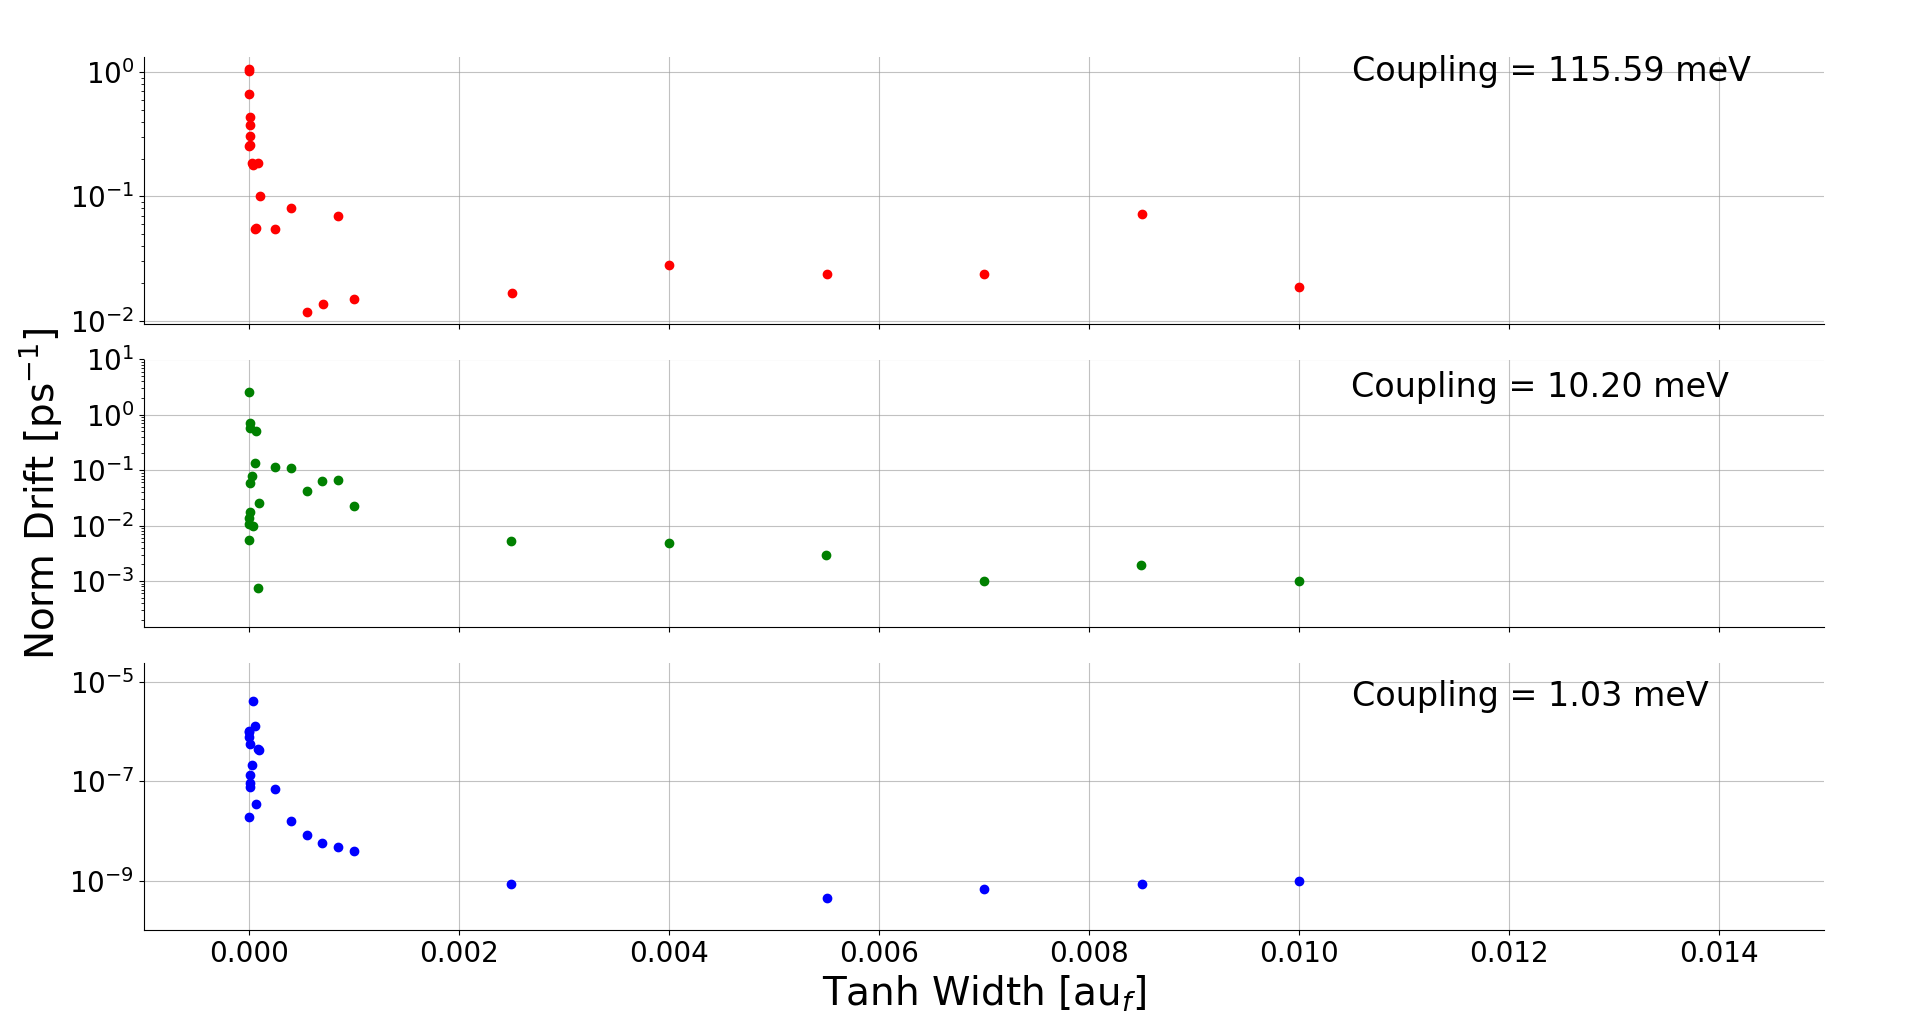
\includegraphics[width=\textwidth]{./img/ManyScaling_NormDriftBetterVersion.png}
  \caption{\label{fig:tanh_result} A figure showing the change in the norm conservation with a varying tanh width for 3 different electronic couplings, 100 meV (top), 10 meV (middle) 1 meV (bottom).}
\end{figure}
\noindent An improvement spanning several orders of magnitude can be seen in figure \ref{fig:tanh_result} for all couplings. However, there is still room for improvement, especially in the higher 2 couplings. Renormalisation at each time-step is necessary to correct small average errors, a more eleborate scheme with a dynamic smoothing width may be required for larger more complex systems.
\\
\subsection{Time-Derivative of the Sum Over Trajectories of Adiabatic Populations}
In the supplementary information of Min, 17 \cite{min_ab_2017} a further condition was imposed when deriving the equation for the Quantum Momentum (equation S26). This is given below:
\begin{equation}
  \sum_{I}^{N_{rep}} \frac{d\vert C_{qm, l}^{(I)} \vert^2}{dt} = \sum_{I}^{N_{rep}} \sum_{\nu}^{N_n} 2 \frac{\mathcal{Q}_{lk, \nu}^{(I)}}{\hbar M_{\nu}} \cdot \left( \textbf{f}_{k, \nu}^{(I)} - \textbf{f}_{l, \nu}^{(I)} \right) \vert C_{l}^{(I)}\vert^2 \vert C_{k}^{(I)}\vert^2 = 0 \qquad \forall l, k
  \label{eq:S26}
\end{equation}
This equation can be used to monitor the dynamics and test the Quantum Momentum calculation. Figure \ref{fig:S26_10meV_0.0001auf} below shows the result of this for an arbitrary coupling (10meV) in a dimer of an Ethylene like molecule.
\begin{figure}[H]
  \includegraphics[width=\textwidth]{./img/Equation_S26/Coup=10meV_Tanh_width=0x0001.png}
  \caption{\label{fig:S26_10meV_0.0001auf}Equation S26 from \cite{min_ab_2017}. A coupling of 10meV was used and a tanh smoothing width was 0.0001 au$_f$.}
\end{figure}
\noindent We can see that the equation is fulfilled to within $\sim 10^{-5}$ with some fairly large spikes. These spikes are caused by a spike in the quantum momentum due to denominator in the $\textbf{R}_{lk, \nu}$ equation \eqref{eq:Rlk} approaching zero. This assures me that the quantum momentum is implemented correctly.


\newpage
